\documentclass[12pt, letterpaper, titlepage]{article}
\usepackage[utf8]{inputenc}
\usepackage{geometry}
\usepackage{color,graphicx,overpic} 
\usepackage{fancyhdr}
\usepackage{amsmath,amsthm,amsfonts,amssymb}
\usepackage{mathtools}
\usepackage{hyperref}
\usepackage{multicol}
\usepackage{array}
\usepackage{float}
\usepackage{blindtext}
\usepackage{longtable}
\usepackage{scrextend}
\usepackage[font=small,labelfont=bf]{caption}
\usepackage[framemethod=tikz]{mdframed}
\usepackage{calc}
\usepackage{titlesec}
\usepackage{listings}
\usepackage[normalem]{ulem}
\usepackage{tabularx}
\usepackage{mathrsfs}
\usepackage{bookmark}
\usepackage{apple_emoji}
\usepackage{setspace}
\usepackage{ragged2e}
\usepackage{ltablex}
\usepackage{textcomp}

% \mathtoolsset{showonlyrefs}  
\allowdisplaybreaks
\lstset{basicstyle=\ttfamily, keywordstyle=\rmfamily\bfseries}

\definecolor{comment}{RGB}{140, 140, 140}
\definecolor{text}{RGB}{0, 0, 0}
\definecolor{string}{rgb}{0.58,0,0}
\definecolor{variable}{RGB}{244, 63, 78}

\lstdefinestyle{customc}{
    frame=L,
    xleftmargin=\parindent,
    belowcaptionskip=1\baselineskip,
    basicstyle=\footnotesize\ttfamily,
    keywordstyle=\bfseries\color{green!40!black},
    commentstyle=\itshape\color{purple!40!black},
    identifierstyle=\color{blue},
    stringstyle=\color{orange},
    breakatwhitespace=false,         
    breaklines=true,                 
    captionpos=b,                    
    keepspaces=true,                 
    numbers=left,                    
    numbersep=-10pt,                  
    showspaces=false,                
    showstringspaces=false,
    showtabs=false,                  
    tabsize=4,
}

\lstset{escapechar=@,style=customc}

\newcolumntype{b}{X}
\newcolumntype{s}{>{\hsize=.25\hsize}X}
\newcolumntype{a}{>{\hsize=.5\hsize}X}

\definecolor{mycolor}{rgb}{0, 0, 0}

\geometry{top=2.54cm, left=2.54cm, right=2.54cm, bottom=2.54cm}
\setlength{\headheight}{20pt}
\setlength{\parskip}{0.3cm}
\setlength{\parindent}{1cm}

\newcommand{\B}{
\includegraphics[height=1.5em, valign=B, raise=-0.2em]{BigB.png}} 

\pagestyle{fancy}
\fancyhf{}
\rhead{\B enjamin Kong | 1573684}
\lhead{\textit{ECE 322 Assignment 5}}
\rfoot{Page \thepage}

\begin{document} 
\onehalfspacing

\section*{Q1}
\subsection*{a)}
The control flow graph for when compound decisions are treated \textit{en bloc} is displayed below. Cyclomatic complexity is 5 resulting from 5 distinct regions.
\begin{figure}[H]
    \centering
    \caption{Control flow graph when compound decisions are treated \textit{en bloc}.}
    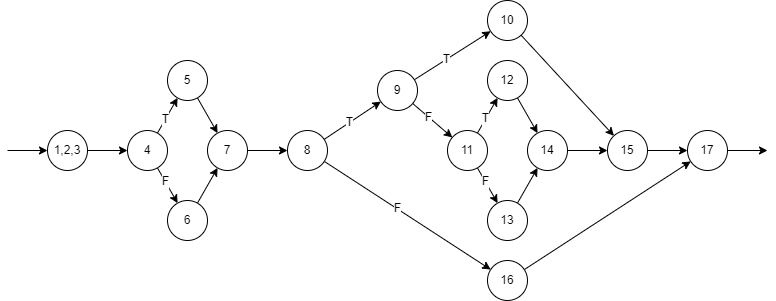
\includegraphics[width=\textwidth]{Q1a.png}
\end{figure}

\subsection*{b)}
The control flow graph for when compound decisions are treated separately is displayed below. Cyclomatic complexity is 10 resulting from 10 distinct regions.
\begin{figure}[H]
    \centering
    \caption{Control flow graph when compound decisions are treated separately.}
    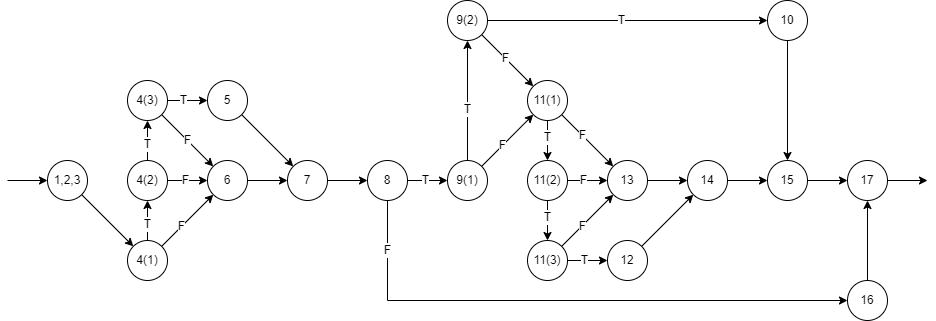
\includegraphics[width=\textwidth]{Q1b.png}
\end{figure}

\section*{Q2}
The code has been translated below. Refer to the line numbers on the left for the control flow graph.
\begin{lstlisting}[language=C++]
    public static double ReturnAverage(int value[], 
                                int AS, int MIN, int MAX) {
        int i, ti, tv, sum;
        double av;
        i = 0; ti = 0; tv = 0; sum = 0;
        while (ti < AS && value[i] != -999) {
            ti++;
            if (value[i] >= MIN && value[i] <= MAX) {
                tv++;
                sum = sum + value[i];
            }
            i++;
        }
        if (tv > 0)
            av = (double)sum / tv;
        else
            av = (double)-999;
        return (av);
    }
\end{lstlisting}

\noindent
The control flow graph is displayed below.
\begin{figure}[H]
    \centering
    \caption{Control flow graph.}
    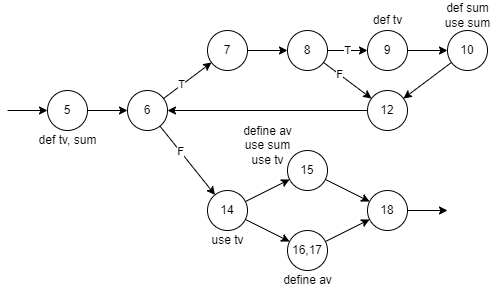
\includegraphics[width=0.75\textwidth]{Q2.png}
\end{figure}

\noindent
Examples of \textit{def-clear} paths are as follows:
\begin{itemize}
    \item $tv$
    \begin{enumerate}
        \item (5, 6, 7, 8)
        \item (9, 10, 12, 6, 14)
        \item (9, 10, 12, 6, 7, 8, 12, 6, 14)
    \end{enumerate}
    \item $av$
    \begin{enumerate}
        \item (15, 18)
        \item (17, 18)
    \end{enumerate}
    \item $sum$
    \begin{enumerate}
        \item (5, 6, 7, 8, 9)
        \item (10, 12, 6, 7, 8, 12, 6, 7, 8)
        \item (5, 6, 7, 8, 12, 6, 7, 8, 9)
    \end{enumerate}
\end{itemize}

\section*{Q3}
\begin{lstlisting}[language=Python]
    def yeet(a):
        x = 0
        y = 0
        if a < 5:
            x = sqrt(a)
            y = a
        else:
            x = a
            y = sqrt(a)
        return x - y
\end{lstlisting}

\newpage

\section*{Q4}
\begin{centering}
\begin{tabularx}{\textwidth}{|X|X|X|X|X|X|}
    \caption{Test cases for ($a || b) \&\& (\text{not}(c) || \text{not}(d))$} \\ \hline
    Test ID & $a$ & $b$ & $c$ & $d$ & Result \\ \hline
    1 & T & F & T & F & T \\ \hline
    2 & T & F & F & T & T \\ \hline
    3 & T & T & T & T & F \\ \hline
    4 & F & F & F & F & F \\ \hline
\end{tabularx}
\end{centering}

\end{document}
